\subsubsection{Hàm Softmax}
Các bài toán phân loại thực tế thường có rất nhiều lớp, mô hình phân loại nhị phân như hồi quy logistic mặc dù có thể áp dụng cho các bài toán đa lớp, chúng vẫn có những hạn chế nhất định, ví dụ như kỹ thuật được sử dụng nhiều nhất là one-vs-rest có một hạn chế về tổng các xác suất.

Hồi quy Softmax hay còn gọi là hồi quy logistic đa thức (Multinomial logistic regression) là phương pháp phân lớp tổng quát hóa mô hình hồi quy logistic cho trường hợp biến đầu ra là đa lớp, giúp khắc phục hạn chế của hồi quy logistic

Ở bài toán phân loại đa lớp, ta cần một mô hình xác suất sao cho với mỗi input $\textbf{x}, a_i$ thể hiện xác suất để input đó rơi vào class $i$. Như vậy cần các $a_i$ phải dương và tổng của chúng bằng $1$. Để có thể thỏa mãn điều kiện này, chúng ta cần nhìn vào mọi giá trị $z_i$ và dựa trên quan hệ giữa các $z_i$ này để tính toán giá trị của $a_i$. Ngoài ra, ta sẽ cần thêm một điều kiện nữa, đó là: giá trị $z_i = \textbf{w}^T_i\textbf{x}$ càng lớn thì xác suất dữ liệu rơi vào class $i$ càng cao, tức là ta cần một hàm đồng biến ở đây.

Lưu ý là $z_i$ có thể nhận giá trị cả âm và dương. Một hàm số mượt đơn giản có thể chắc chắn biến $z_i$ thành một giá trị dương, và đồng biến, là hàm $\text{exp}(z_i) = e^{z_i}$. Điều kiện mượt để thuận lợi hơn trong việc tính đạo hàm sau này, và tổng các $a_i$ bằng 1 có thể được đảm bảo nếu:
\begin{equation*}
    a_i = \frac{\text{exp}(z_i)}{\sum^C_{j=1}\text{exp}(z_j)}, \forall i = 1,2,\dots,C
\end{equation*}

Hàm số trên được gọi là hàm \emph{Softmax}. Với cách định nghĩa này, không có xác suất $a_i$ nào tuyệt đối bằng $0$ hoặc $1$.
Lúc này ta giả sử rằng:
\begin{equation*}
    P(y_k =i|\textbf{x}_k;\textbf{W}) = a_i
\end{equation*}

Trong đó, $P(y=i|\textbf{x};\textbf{W})$ là xác suất để một điểm dữ liệu $\textbf(x)$ rơi vào lớp thứ $i$ nếu biết tham số là $\textbf{W}$

\begin{figure}[h!]
    \centering
    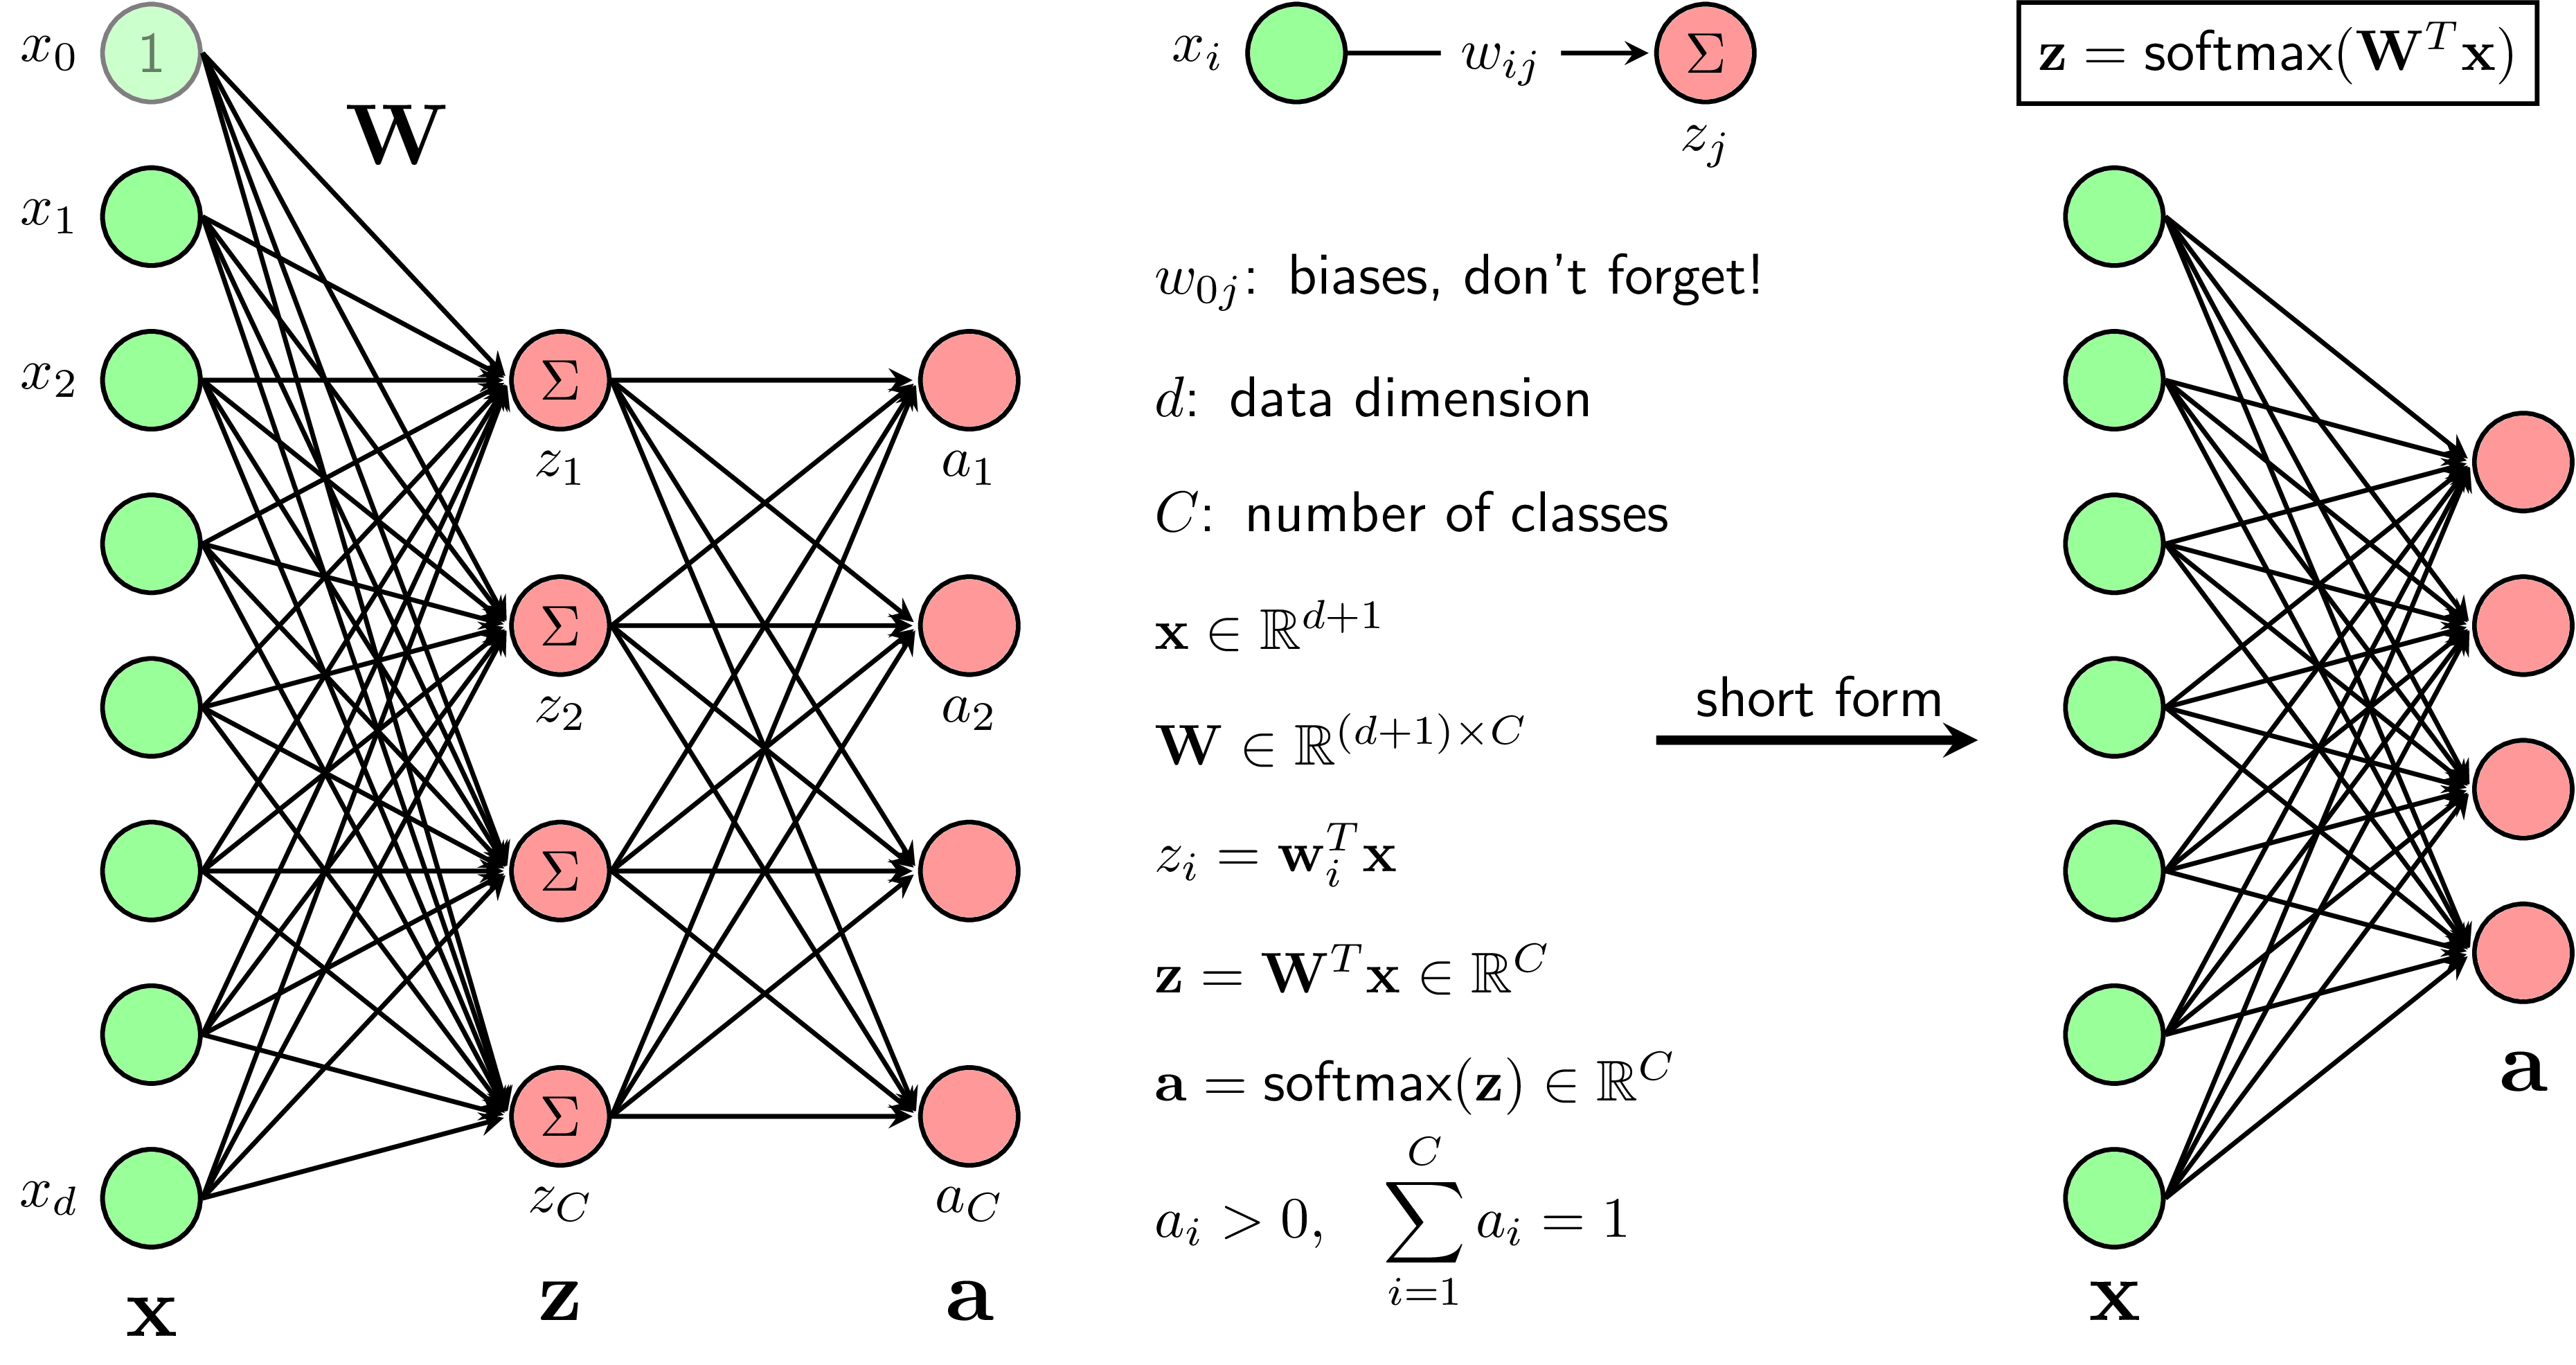
\includegraphics[width=1\textwidth]{figures/softmax_nn.png} % độ rộng ảnh bằng 0.6 độ rộng tối đa của một dòng
    \caption{Mô hình hồi quy Softmax dưới dạng mạng nơ ron} % caption của ảnh
    \label{fig:1} % label của ảnh dùng để reference ảnh. Trong bài viết có chỗ nào cần nói "tại hình 1" thì viết "tại hình \ref{fig:1}"
\end{figure}

Ở phần bên phải, hàm tuyến tính $\sum$ và hàm \emph{softmax} được tách riêng ra để phục vụ cho mục đích minh họa. Dạng short form ở bên phải là dạng hay được sử dụng trong các mạng nơ ron, lớp $\textbf{a}$ được ngầm hiểu là bao gồm cả lớp $\textbf{z}$.

\subsubsection{Hàm mất mát và tối ưu}

Hàm mất mát được sử dụng cho mô hình hồi quy Softmax là \emph{Cross Entropy}.
Cross entropy giữa hai phân phối $p$ và $q$ được viết như sau:
\begin{equation*}
    \textbf{H}(\textbf{p},\textbf{q}) = - \sum^C_{i=1}p_ilogq_i
\end{equation*}
Với hồi quy Softmax, trong trường hợp có $C$ lớp, mất mát giữa đầu ra dự đoán và đầu ra thực sự của dữ liệu $\textbf{x}_i$ được tính như sau:
\begin{equation*}
    \textbf{J}(\textbf{W};\textbf{x}_i;\textbf{y}_i) = - \sum^C_{j=1}y_{ij}log(a_{ij})
\end{equation*}

Với $y_{ij}$ và $a_{ij}$ lần lượt là phần tử thứ $j$ của véc tơ $\textbf{y}_i$ và $\textbf{a}_i$.

Kết hợp tất cả các cặp dữ liệu $\textbf{x}_i, \textbf{y}_i, i = 1,2,\dots,N$, ta sẽ có hàm mất mát của Hồi quy Softmax:
\begin{equation*}
    \textbf{J}(\textbf{W};\textbf{X},\textbf{Y}) = - \sum^N_{i=1}\sum^C_{j=1}y_{ij}log(a_{ij}) = - \sum^N_{i=1}\sum^C_{j=1}y_{ij}log\Big(\frac{\text{exp}(\textbf{w}^T_j\textbf{x}_i)}{\sum^C_{k=1}\text{exp}(\textbf{w}^T_k\textbf{x}_i)}\Big)
\end{equation*}

Việc tối ưu hàm mất mát sẽ sử dụng phương pháp tối ưu theo gradient, ví dụ ở đây ta sử dụng Stochastic Gradient Descent (SGD).
Với mỗi cặp dữ liệu $(\textbf(x)_i, \textbf(y)_i)$ ta có:
\begin{equation} \label{eq:1}
    \textbf{J}_i(\textbf{W}) \stackrel{\bigtriangleup}{=} \textbf{J}(\textbf{W};\textbf{x}_i,\textbf{y}_i) = - \sum^C_{j=1}y_{ij}log\Big(\frac{\text{exp}(\textbf{w}^T_j\textbf{x}_i)}{\sum^C_{k=1}\text{exp}(\textbf{w}^T_k\textbf{x}_i)}\Big) = - \sum^C_{j=1}y_{ji}\textbf{w}^T_j\textbf{x}_i + log\Big(\sum^C_{k=1}\text{exp}(\textbf{w}^T_k\textbf{x}_i)\Big)
\end{equation}

Tiếp theo ta sử dụng công thức:
\begin{equation} \label{eq:2}
    \frac{\partial\textbf{J}_i(\textbf{W})}{\partial\textbf{W}} = \Bigg[\frac{\partial\textbf{J}_i(\textbf{W})}{\partial\textbf{w}_1}, \frac{\partial\textbf{J}_i(\textbf{W})}{\partial\textbf{w}_2},\dots,\frac{\partial\textbf{J}_i(\textbf{W})}{\partial\textbf{w}_C}\Bigg]
\end{equation}

Trong đó gradient từng cột có thể tính dựa theo công thức \ref{eq:1}:
\begin{equation}  \label{eq:3}
    \frac{\partial\textbf{J}_i(\textbf{W})}{\partial\textbf{w}_j} = -y_{ji}\textbf{x}_i + \frac{\text{exp}(\textbf{w}^T_j\textbf{x}_i)}{\sum^C_{k=1}\text{exp}(\textbf{w}^T_k\textbf{x}_i)}\textbf{x}_i = -y_{ji}\textbf{x}_i + a_{ji}\textbf{x}_i = \textbf{x}_i(a_{ị}-y_{ji}) = e_{ji}\textbf{x}_i
\end{equation}

Kết hợp \ref{eq:2} và \ref{eq:3} ta có:
\begin{equation*}
    \frac{\partial\textbf{J}_i(\textbf{W})}{\partial\textbf{W}} = \textbf{x}_i[e_{1i},e_{2i},
    \dots,e_{Ci}] = \textbf{x}_i\textbf{e}^T_i
\end{equation*}

Từ đó suy ra:
\begin{equation*}
     \frac{\partial\textbf{J}(\textbf{W})}{\partial\textbf{W}} = \sum^N_{i=1}\textbf{x}_i\textbf{e}^T_i = \textbf{X}\textbf{E}^T
\end{equation*}